
%%%%%%%%% MASTER -- compiles the 4 sections

\documentclass[11pt,letterpaper]{article}

\usepackage{graphicx}
\usepackage{verbatim}
\usepackage{listings}
%%%%%%%%%%%%%%%%%%%%%%%%%%%%%%%%%%%%%%%%%%%%%%%%%%%%%%%%%%%%%%%%%%%%%%%%%
\pagestyle{plain}                                                      %%
%%%%%%%%%% EXACT 1in MARGINS %%%%%%%                                   %%
\setlength{\textwidth}{6.5in}     %%                                   %%
\setlength{\oddsidemargin}{0in}   %% (It is recommended that you       %%
\setlength{\evensidemargin}{0in}  %%  not change these parameters,     %%
\setlength{\textheight}{8.5in}    %%  at the risk of having your       %%
\setlength{\topmargin}{0in}       %%  proposal dismissed on the basis  %%
\setlength{\headheight}{0in}      %%  of incorrect formatting!!!)      %%
\setlength{\headsep}{0in}         %%                                   %%
\setlength{\footskip}{.5in}       %%                                   %%
%%%%%%%%%%%%%%%%%%%%%%%%%%%%%%%%%%%%                                   %%
\newcommand{\required}[1]{\section*{\hfil #1\hfil}}                    %%
\renewcommand{\refname}{\hfil References Cited\hfil}                   %%
\bibliographystyle{plain}                                              %%
%%%%%%%%%%%%%%%%%%%%%%%%%%%%%%%%%%%%%%%%%%%%%%%%%%%%%%%%%%%%%%%%%%%%%%%%%

%PUT YOUR MACROS HERE

\date{December 14th, 2011}
\title{Evolutionary Computation\\
in Muscle Action Simulations
}

\author{Colby Blair \\
	Computer Science Undergraduate \\
	University of Idaho Computer Science Department
}

\begin{document}
\maketitle

\begin{abstract}
In biomechanics, there are many interactions between the body and brain. Some
interactions can be quantified as electrical signals to motor nerves of muscles.
The result is a particular musclular reaction due to an electrical signal. The
input is an electrical nerve signal, and the output is a measured velocity at
a joint. The overall result to this sytem of inputs and output is actions like 
walking.

In this project, a Genetic Algorithm (GA) is used to replace the Simulated Annealing (SA) optimization
that Dr. Craig McGowan uses for his research in biomechanics. His research takes EMG signals as inputs,
and tries to predict joint velocities as outputs. This report shows that the GA is much slower, but 
maintains better solutions when it is set up with the right parameters. This report will also recommend
further research opportunities for better results and performance.
\end{abstract}

\thispagestyle{empty}


\pagebreak

\thispagestyle{empty}
\tableofcontents
\listoffigures

\pagebreak

\setcounter{page}{1}
\section{Introduction}
Walking requires a lot of complex tasks to make locomotion possible 
\cite{mcgowan}. The inputs to muscle motor nerves and the outputs of joint
motion are one way of measuring all these complex tasks. The data collected
as inputs and outputs fits nicely into Evolutionary Computation (EC). EC uses 
many measured inputs and expected outputs, and evolves a system that will 
produce those expected outputs on its own. 

The EC program will do this with some margin of error, of course, but the 
error of the solution should be small. The EC solution will then be useful 
when there are a set of inputs that the output is not already know, like in 
a simulation. In this report, we will use a \textbf{Genetic Program (GA)} as
it fits the multiple input to one output model well. The expected output is 
used to evaluate the GA individuals using a fitness function. This fitness 
function calls the muscle simulation function with paramaters help by each
GA individual. These parameters are changed in a scheme discribed next, and
the individuals' fitnesses depend on how well their parameters do in the 
simulation.

\subsection{Hypothesis}
As noted above, the GA is set up to represent SA as closely as possible,
at least at first. Our hypothesis is that the GA will find better solutions
than the SA, while having the advantage of trying more diverse solution that
would could cause worse solutions for an SA. The GA will be able to better
search the domain, without as many problem with local optimums. These 
advantages may come at the cost of process time, but are hypothesized to 
not be significant.

%%%%%%%%% PROPOSAL -- 15 pages (including Prior NSF Support)
% From the NSF Grants Proposal Guide:
% "The Project Description should provide a clear statement of the work 
% to be undertaken and must include: objectives for the period of the proposed 
% work and expected significance; relation to longer-term goals of the PI's 
% project; and relation to the present state of knowledge in the field, 
% to work in progress by the PI under other support and to work in progress 
% elsewhere."

%\required{Project Description}
\section{Project Description}

\subsection{Agenda}

\subsubsection{Algorithms / Programming}

\begin{figure}[!h]
        \begin{center}
		%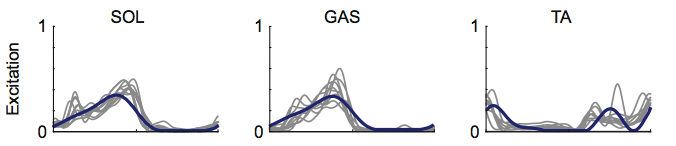
\includegraphics[width=120mm]{images/excite}
                \caption{Some great figure}
                \label{curves}
        \end{center}
\end{figure}


\subsection{Methodology}
%this section should talk about how the team will develop, maybe software
% processes, and how to get customer feedback

\subsubsection{Project Software}
TODO: This project will be written in Ruby on Rails or some other great 
MVC, will install on Windows, Linux, and Mac, blah blah blah. It will be 
downloadable to customers via a private github, Apple's App Store,
or some other overpriced method. Consulting to set it up won't exist because
the whole thing installs itself, and everything is so simple. 

\section{Customer}
%Talk about Alex and the Methow, and all the doe they are rolling in to pay
% for this thing.
%Talk about their needs, and the impact this project could have on them.
%Talk also about how future customer, not just in the Basin, but elsewhere
% could benefit from the product.

\section{Statement of Qualifications}
%What gives us the idea we can actually pull this off?

\section{Conclusion}
%Why should people pay for this thing, why should the capstone PM's want
% this project, and why is it great for humanity


%\required{Broader Impacts}
% as in the project summary, broader impacts must be called out separately 
% in the project description.  You may be able to give more specific
% examples, or discuss how you've previously achieved these impacts.
% It should be similar, but not identical, to the Broader Impacts statement
% in the project summary

%\required{Results From Prior NSF Support}
% 5 pages or fewer of the 15 pages for entire description document.
% include results from NSF grants received in the past 5 years.
% if supported by more than one grant, choose the most relevant one
% for each grant, include: NSF award number, amount, dates of
% support, and publications resulting from this research.
% due to space limitations, it is often advisable to use citations rather
% than putting the titles of the publications in the body 
% of this section

% e.g.: "My prior grant, "Uses of Coffee in Mathematical Research" (DMS-0123456, 
% $100,000, 2005-2008), resulted in 3 papers [1],[2],[3], demonstrating..."

% if requesting postdoctoral research salary, a supplemental 1-page document
% called "Postdoc Mentoring Plan" will be required 


\section{Results}

\subsection{Simulated Annealing}
This section lists some SA optimizations for comparison.

\subsubsection{Run 1} 
\label{sec:run_1}

\begin{tabular}{lr}
	Min: 			& 127030005662992 \\
	Max:			& 1636549083561452 \\
	Standard Deviation:	& 217723255965676\\
\end{tabular}

\begin{figure}[!h]
	\begin{center}
		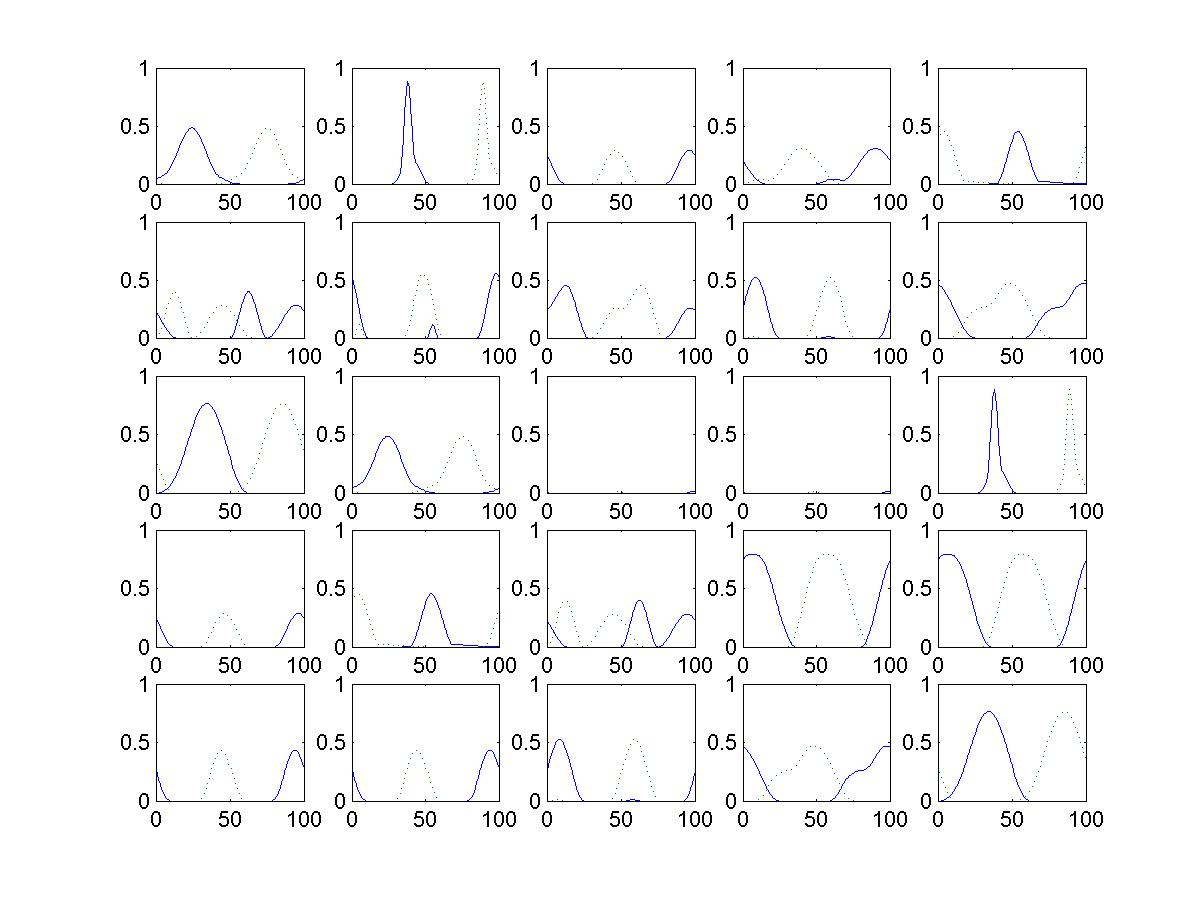
\includegraphics[width=120mm]{images/saXX_exc}
               	\caption{SA muscle excitation patterns}
                \label{saXX_exc}
        \end{center}
\end{figure}

\pagebreak
\begin{figure}[!h]
	\begin{center}
		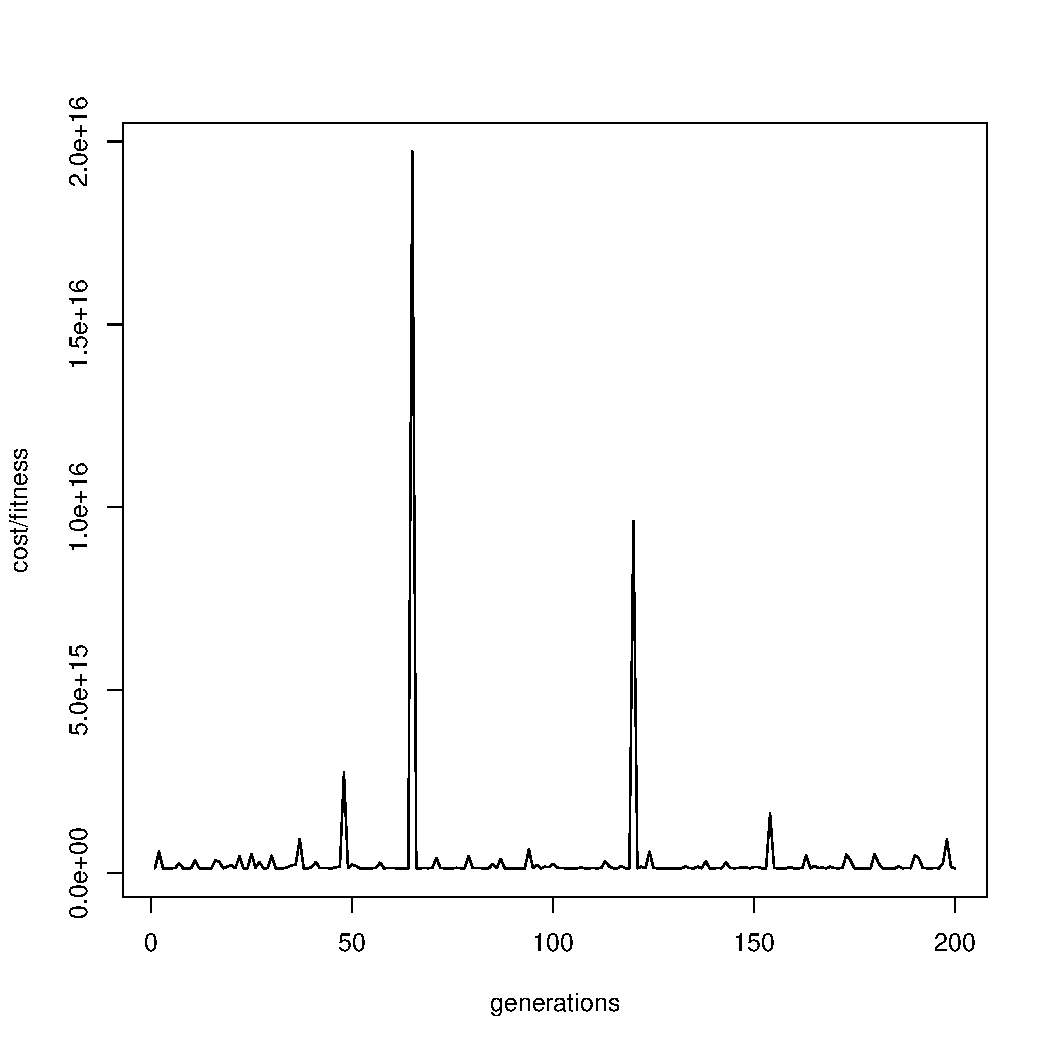
\includegraphics[width=120mm]{output/sa01/graph_all.pdf}
               	\caption{SA fitness over generations}
                \label{saXX_exc}
        \end{center}
\end{figure}

\pagebreak
\begin{figure}[!h]
	\begin{center}
		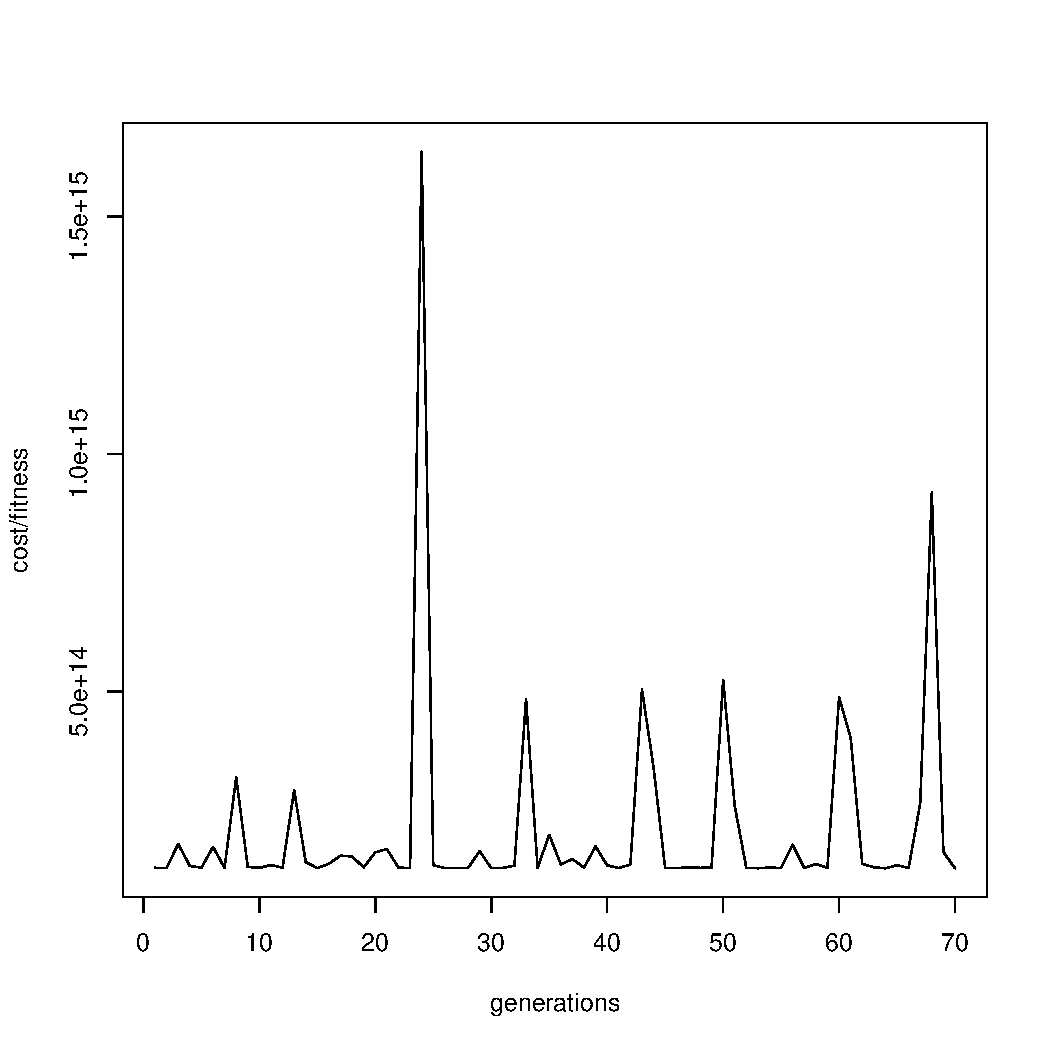
\includegraphics[width=120mm]{output/sa01/graph_70.pdf}
               	\caption{Same SA fitness over last 70 generations}
                \label{sa01_70_exc}
        \end{center}
\end{figure}

\pagebreak

\subsection{Genetic Algorithm with Mutation Only}

\subsubsection{GA Run 1}
\begin{tabular}{lr}
	Min: 			& 127156943557514  \\
	Max:			& 127354767955212  \\
	Standard Deviation:	& 35435274465.6039 \\
\end{tabular}

Parameters for ga:\\
\begin{tabular}{lr}
	POP\_SIZE:	& 10 \\
	ATTR\_SIZE:	& 96 \\
	GA\_LBOUND:	& -5.000 \\
	GA\_UBOUND:	& 100.00 \\
	GA\_DIFF\_SCALE: & 800.000 \\
	K\_MUT:		& 96 \\
	K\_SELECT:	& 1 \\
\end{tabular}

\begin{figure}[!h]
	\begin{center}
		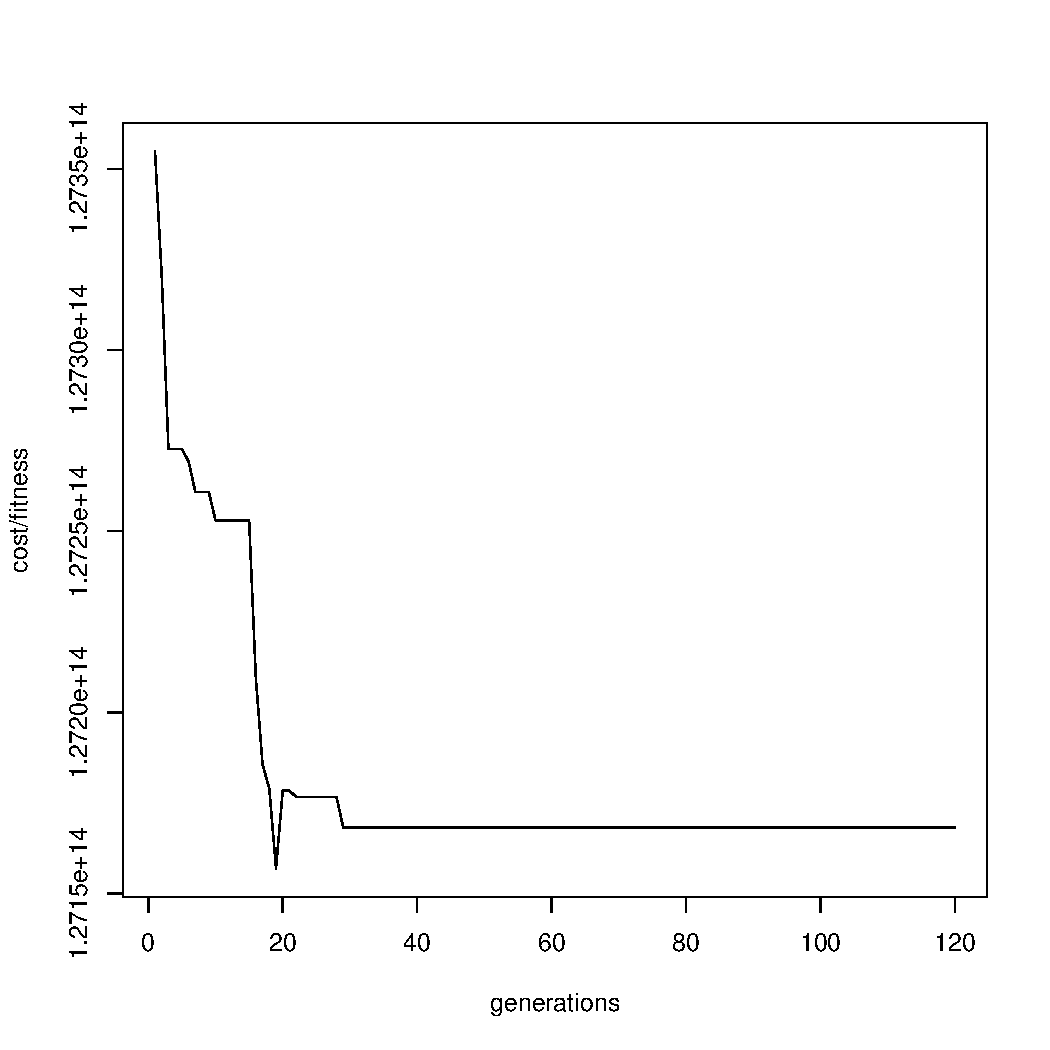
\includegraphics[width=120mm]{output/ga01/graph.pdf}
               	\caption{GA fitness, uniform mutation only}
                \label{ga01_exc}
        \end{center}
\end{figure}

\pagebreak
\subsubsection{GA Run 2}
\begin{tabular}{lr}
	Min: 			& 126393050706189   \\
	Max:			& 126471924413236   \\
	Standard Deviation:	& 24842647883.601  \\
\end{tabular}


Parameters for ga:\\
\begin{tabular}{lr}
	POP\_SIZE:	& 10 \\
	ATTR\_SIZE:	& 96 \\
	GA\_LBOUND:	& -5.000 \\
	GA\_UBOUND:	& 100.00 \\
	GA\_DIFF\_SCALE: & 800.000 \\
	K\_MUT:		& 96 \\
	K\_SELECT:	& 1 \\
\end{tabular}

\begin{figure}[!h]
	\begin{center}
		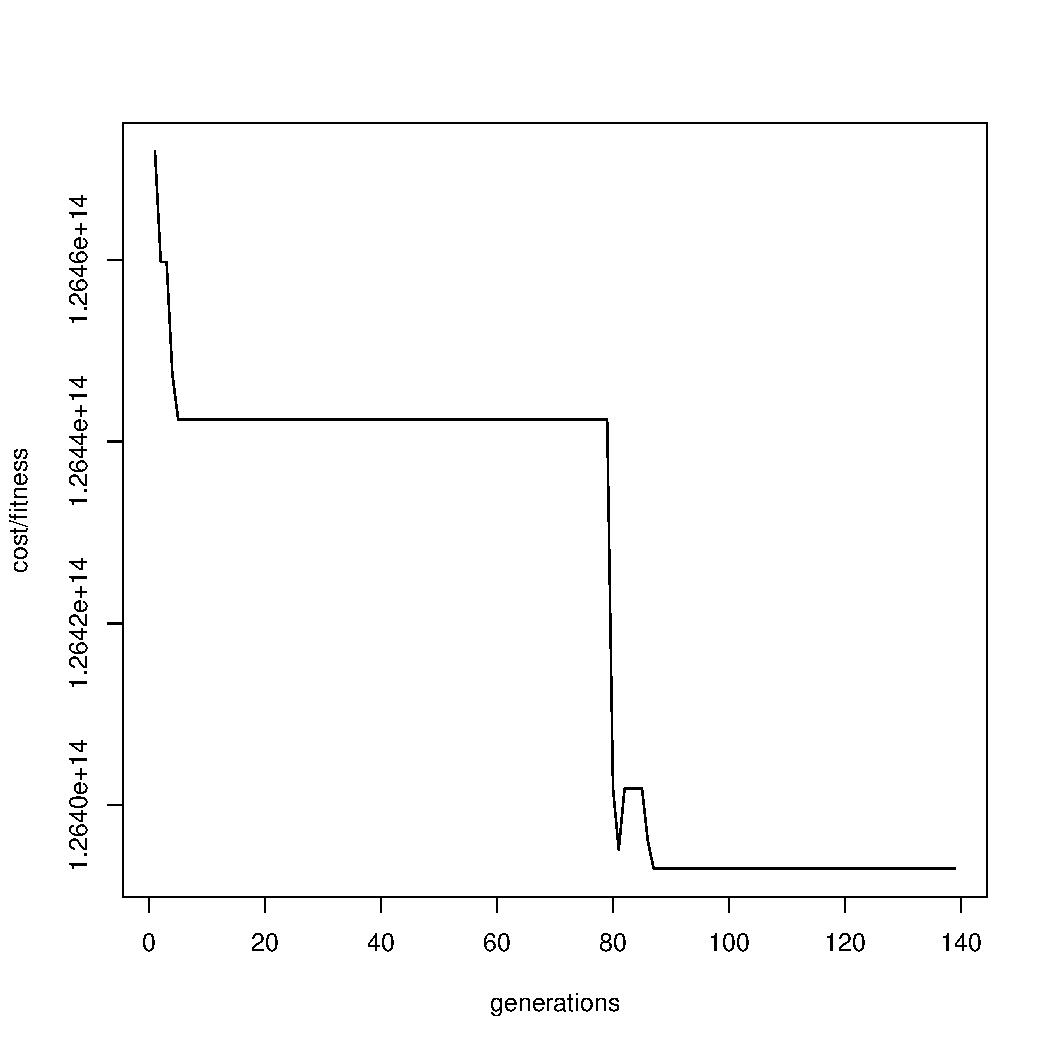
\includegraphics[width=120mm]{output/ga02/graph.pdf}
               	\caption{Another GA fitness, uniform mutation only}
                \label{saXX_exc}
        \end{center}
\end{figure}

\pagebreak
\subsection{Genetic Algorithm with Uniform Mutation and Point Crossover}
\subsubsection{GA Run 3}
\begin{tabular}{lr}
	Min: 			& 126286311965193 \\
	Max:			& 126903624988318 \\
	Standard Deviation:	& 226416086588.11 \\
\end{tabular}

Parameters for ga:\\
\begin{tabular}{lr}
	POP\_SIZE:	& 10 \\
	ATTR\_SIZE:	& 96 \\
	GA\_LBOUND:	& -5.000 \\
	GA\_UBOUND:	& 100.00 \\
	GA\_DIFF\_SCALE: & 800.000 \\
	K\_MUT:		& 96 \\
	K\_SELECT:	& 1 \\
	K\_FLIP\_XOVER:	& 1 \\
\end{tabular}

\begin{figure}[!h]
	\begin{center}
		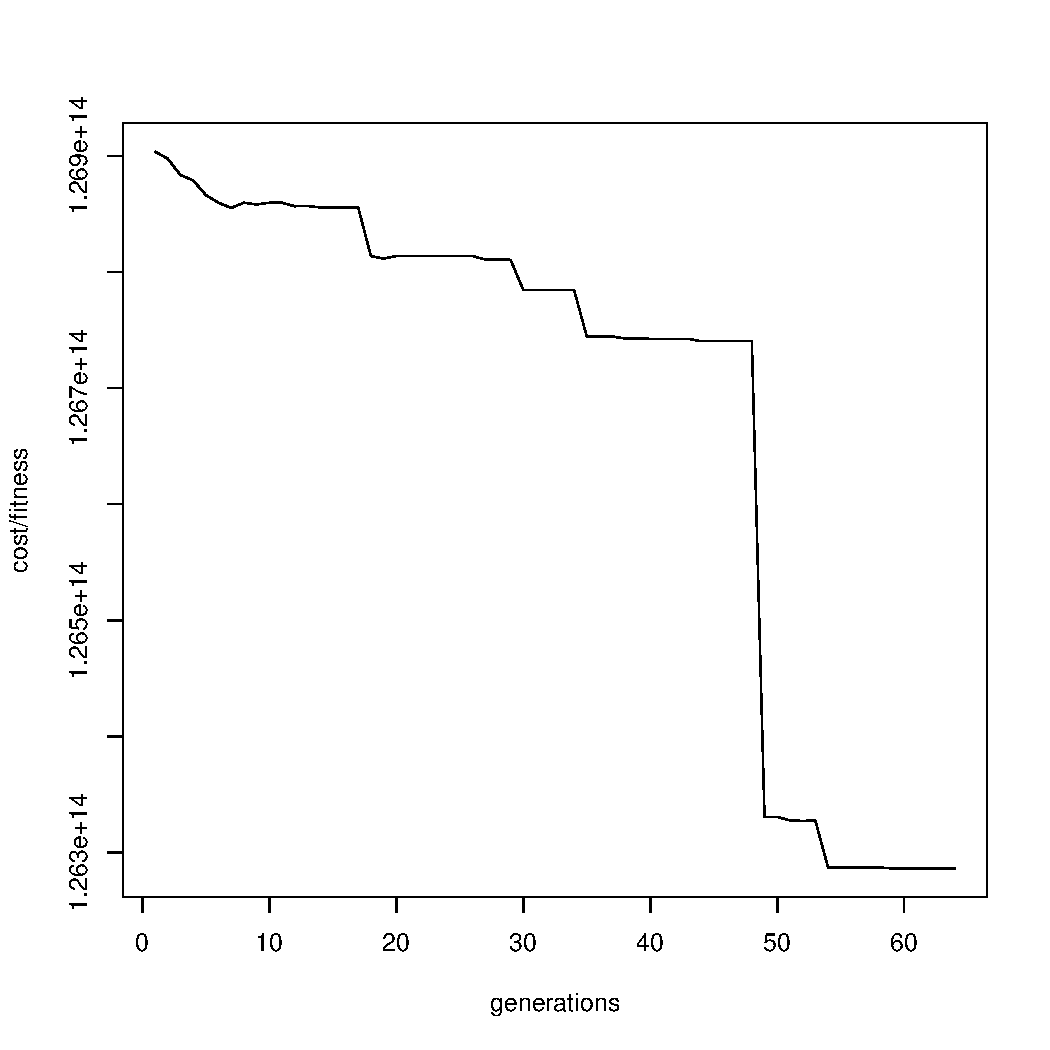
\includegraphics[width=120mm]{output/ga03/graph.pdf}
               	\caption{GA fitness, uniform mutation and one point flip crossover}
                \label{saXX_exc}
        \end{center}
\end{figure}


\subsection{Algorithm Comparison}
\begin{tabular}{llll}
Optimization	& Min			& Max			& Standard Deviation \\
SA		& 127030005662992 	& 1636549083561452	& 217723255965676 \\
GA Run 1	& 127156943557514	& 127354767955212	& 35435274465.6039 \\
GA Run 2	& 126393050706189	& 126471924413236	& 24842647883.601 \\
GA Run 3	& 126286311965193	& 126903624988318	& 226416086588.11 \\
\end{tabular}

\section{Performance}
The overhead of both the SA and the GA are almost nothing ( $\le .01$ second per
iteration / generation). Especially compared to the cost / fitness function,
which has to run the simulation every time to get results. The main 
disadvantage of the GA over the SA is that for every iteration, it has to run
the simulation function once for every individual in the population. For this
project, the population size was 10, so the GA was approximately 10 times
as slow as the SA.

The good thing about the slowdown, is that it happens in data independent
region of the process; each fitness iteration for each individual can be 
calculated without needing to share data with other iterations. This meets the
criteria for true \textbf{task parallelism}, or running each fitness function
simultaneously.

\subsection{Enhancements with Parallelism}
To understand parallelism and the gains from it, we must consider Amdahl's Law:
\begin{figure}[h]
	\begin{center}
		\LARGE
		\begin{tabular}{l r}
			$ A $		&	$ = \frac{1}{(1 - P) + \frac{P}{N}} $ \\
		\end{tabular}

		\normalsize
		\begin{tabular}{l l}
			$ where $  & \\
					&	$ P $ is the portion of the program that can be 'parallelized' \\
					&	$ N $ processors or workers \\
					&	$ (1 - P) $ is the sequential / serial portion (cannot be parallelized) \\
		\end{tabular}
		\caption{Amdah's Law. \cite{amdahl}} 
		\label{amdahl}
	\end{center}
\end{figure}
\normalsize

$ P $ informally is the portion of the program that can be split up into sections, each of which can be worked 
on simultaniously. The name for this process is \textbf{paralellization}. Informally, Ahmdahl's Law shows that 
the higher $ P $, or portion of work that can be split up, the more beneficial adding more CPU's ($ N $) is. Too many CPU's, and the benefit decreases.

For parallelism over many CPU's on a network, an API like OpenMPI can be used.
This creates an additional element, and that is the time cost of moving data
over the network:

\begin{figure}[h]
	\begin{center}
		\LARGE
		\begin{tabular}{l r}
			$ A $	&	$ = \frac{1}{((1 - P) + (T_P * N)) + \frac{P}{N}} $ \\
		\end{tabular}

		\normalsize
		\begin{tabular}{l l}
			$ where $  & \\
				&	$ P $ is the portion of the program that can be 'parallelized' \\
				&	$ N $ processors or workers \\
				&	$ (1 - P) $ is the sequential / serial portion (cannot be parallelized) \\
				&	$ (T_P * N) $ is the overhead \\
		\end{tabular}
		\caption{Amdah's Law (Figure \ref{amdahl}) with Overhead. } 
		\label{amdahl_overhead}
	\end{center}
\end{figure}
\normalsize

Adding more CPU's actual slows parallel processes down at a certain point.
For many algorithms, $ P $ can only be a fairly small size. The best value for $ N $ will then only be 1. If $ P $ is not very big to begin with, than any $ N $ greater than 1 will cause a slowdown instead 
of speedup. Thus, even though some programs can be parallelized, if $ N > 1 $ causes a slowdown, they shouldn't.

For the muscle excitation GA, we luckily have a fairly high $ P = 13.10 $
seconds,  and a low $ T_P = .08 $ seconds. $ P $ is the measured time for each
simulation to run, and $ T_P $ is an approximation of how long the data takes
to travel across an MPI network. The resulting graph for speed is below:

\begin{figure}[!h]
	\begin{center}
		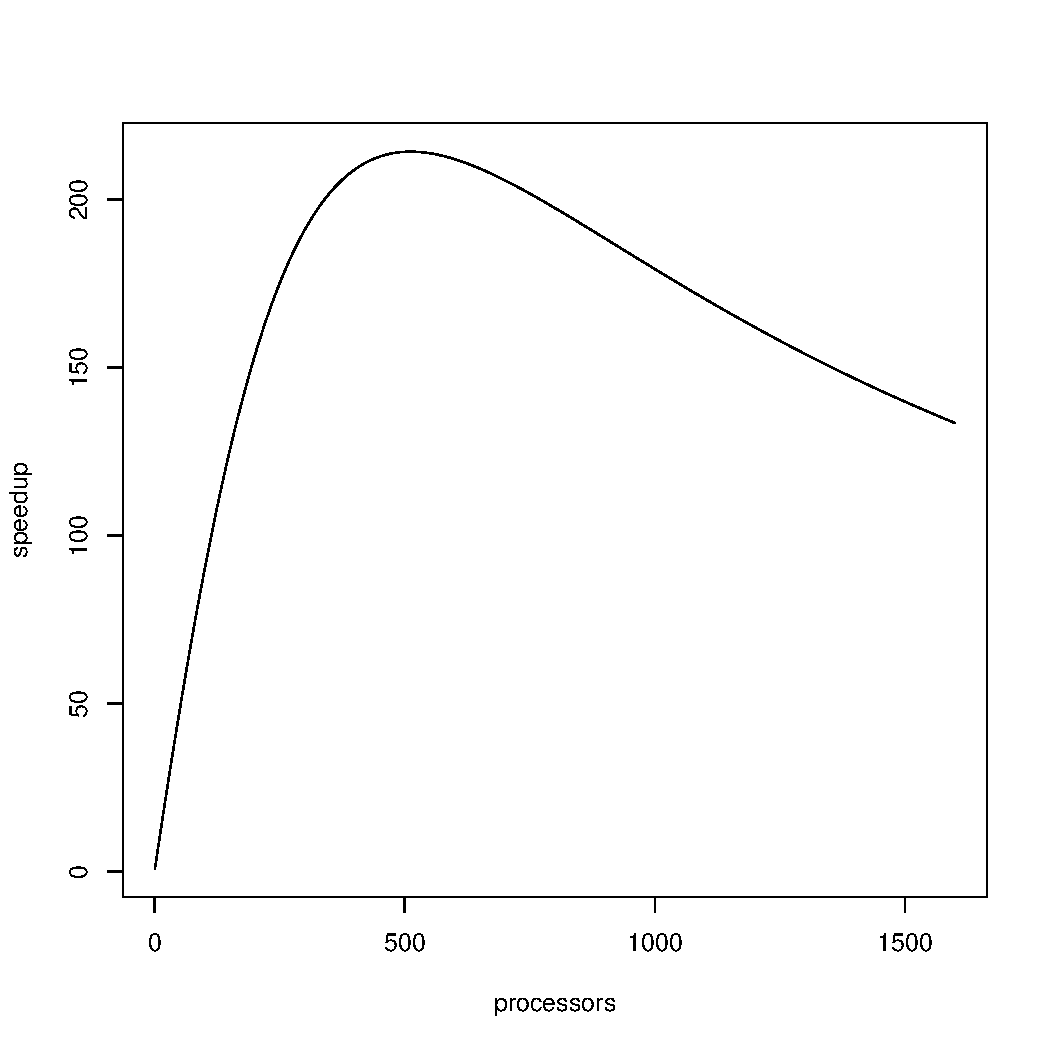
\includegraphics[width=120mm]{images/amdahl_graph.pdf}
               	\caption{Proposed speedup using OpenMPI and Amdahl's Law with Overhead (Figure \ref{amdahl_overhead}) }
                \label{speedup}
        \end{center}
\end{figure}

In figure \ref{speedup}, observe that the max speedup is 214.264919941776 with 
512 CPU's. Although this is the most speedup, significantly less will give more 
speedup for the extra cost, and a small to medium size computing cluster 
(50-100+ CPU's) would be very beneficial.

\section{Conclusion}
In conclusion, the GA outperformed the SA a little bit at the cost of a lot
of extra compute time. This may be still desirable, if the GA is in fact
exploring a global optimum. It is probable, however, that there is a very 
sudden global optimum somewhere, and this GA doesn't maintain enough diversity
to find it.

The project started with trying to imitate an SA using a GA, and then added 
more variability with mutation and crossover rates. What was quite suprising
was how sensitive the existing solution were to mutation and crossover.
The solutions the GA started with were recent bests found by the SA, and 
the GA originally changed them so much that fitness / cost went to infinity.
This is why this project used such conservative changes, scaling down 
mutations 800 times (Figure \ref{uniform_mutation}) and even leaving out 
crossover (Section \ref{sec:run_1}). When we did use crossover, it was very
conservative flip crossover, like flipping only 1, 2, or 3 attributes 
between individuals.

This conservation could be because the GA is already stuck in a local optimum,
and we have pressured it hard to not stray outside. It may also be that the 
fitness function is a little inaccurate.

In this report, it was hypothesized that the GA would find a better solution
through diversity. Instead, this GA found a better solution within the search
space that the SA was probably already searching. To get the GA to try more 
diverse solutions, it may be necessary to start the simulations without
initial solutions already found by the SA. We also hypothesized not much
performance difference between the SA and GA, but once we found out the
simulation time, this was definitely not true.

This GA found better solutions in our limited testing, but could probably
be better. Implementing the performance enhancements suggested may be the only
way to try larger populations, and to try more parameters for the GA.

Finally, it should be said that these parameters for the GA could easily be
controlled by another GA, or meta-GA. Even a GA for the fitness function
may be a good idea, as Dr. McGowan's current research edits this by hand.
There is a lot of opportunity for improvement, and hopefully some of the 
things found here will be useful in future research.

\section{Source}
These file have .cpp postfixes, but were originally written in C, and take
a C style. The development environment was Visual Studio C++, and with a 
better understanding of it, these files will go back to being pure C.

\subsection{ga\_main.h}
\lstinputlisting{src/Walking_Simulation_latest/src/ga_main.h}

\subsection{ga\_main.cpp}
\lstinputlisting{src/Walking_Simulation_latest/src/ga_main.cpp}

\subsection{ga\_i.h}
\lstinputlisting{src/Walking_Simulation_latest/src/ga_i.h}

\subsection{ga\_i.cpp}
\lstinputlisting{src/Walking_Simulation_latest/src/ga_i.cpp}

\subsection{ga\_pop.h}
\lstinputlisting{src/Walking_Simulation_latest/src/ga_pop.h}

\subsection{ga\_pop.cpp}
\lstinputlisting{src/Walking_Simulation_latest/src/ga_pop.cpp}


%%%%%%%%% REFERENCES -- no limit

% this should include only items referenced in the project description
% it is not a bibliography of related reading.

% Each reference must include the names of all authors (in the same
% sequence in which they appear in the publication), the article and 
% journal title, book title, volume number, page numbers, and year of 
% publication. If the document is available electronically, the website 
% address also should be identified

\section{Bibliography}

\begin{thebibliography}{99}
\bibitem{mcgowan} Neptune, R.R.; McGowan, C.P. 
	"Muscle contributions to whole-body sagittal plane angular momentum during walking" 
	{ \em Journal of Biomechanics, 2011 }. 44 6–12 : Print.
\bibitem{amdahl} Amdahl, Gene (1967). "Validity of the Single Processor Approach to Achieving Large-Scale Computing Capabilities". {\em AFIPS Conference Proceedings} (30): 483–485. Print.
\bibitem{thelen} Thelen, D.G.; Anderson, F.C. "Using computed muscle control to generate forward dynamic simulations of human walking from experimental data"
	{ \em Journal of Biomechanics, 2006 }. 39 1107 - 1115: Print.
\bibitem{lloyd} Lloyd, G.L.; Besier, T. F.
	"An EMG-driven musculoskeletal model to estimate muscle forces and knee joint moments in vivo"
	{ \em  Journal of Biomechanics, 2003 }. 36 765-776: Print.
\end{thebibliography}

%
%%%%%%%%% BIOGRAPHICAL SKETCH -- 2 pages

\required{Biographical Sketch: Your Name}

% Your Bio should be divided into the following sections
% (a) Professional Preparation (education):
% Undergrad, Major, Year
% Graduate, Major, Year
% Postdoc, Area, Years-Inclusive
% (b) Appointments:  most recent first.
% (c) Publications:  5 related to the proposal, and 5 "Other Significant Publications"
% (d) Synergistic Activities (math-enhancing activities that were not
% part of your main job description, like editorial boards and
% conference organizing - any Math-related volunteer work.
% these are often similar to Broader Impacts

% (e) Collaborators & Other Affiliations: (use the following sections)
% list in alphabetical order, and include current affiliations parenthetically
% Collaborators and Co-editors: past 48 months.  If none, write "none"
% Graduate Advisors and Postdoctoral sponsors: (your own, no matter how long ago)
% Thesis advisor and postgraduate scholar-sponsor:  those you have advised
% in the past 5 years.  
% Total number of graduate students advised: X (all time)
% Total number of postdoctoral scholars sponsored: Y (all time)






\end{document}
